% Pour toute question sur l'utilisation de cette classe, écrivez à jerome.soucy(at)ulaval.ca
% Nécessite la classe Evaluation.sty dans le même dossier ou dans le PATH de votre système
% Nécessite le fichier logo_ul.pdf dans le même dossier un dans le PATH de votre système
\def\Ponderation{30}
\def\SigleNumero{STT-2100}
\def\NomCours{Régression}
\def\DateEvaluation{15 octobre 2024}
\def\DateRemise{}
\def\HeureRemise{}
\def\HeureEvaluation{8h30 à 10h20}
\def\Session{Été 2021}
\def\NomEvaluation{Examen 1}

% Ne rien mettre entre les accolades si l'enseignant (ou l'enseignante) est aussi le coordonnateur (ou la coordonnatrice)
\def\Coordonnatrice{}
\def\Coordonnateur{}

% Ne rien mettre entre les accolades s'il y a plus d'une section
\def\Enseignant{}
\def\Enseignante{Audrey-Anne Vallée}

% Ne rien mettre entre les accolades s'il s'agit d'un cours à section unique
% Mettre le nom de chacun des enseignants et enseignantes entre les accolades
% Une case à cocher sera générée pour chacune des sections
\def\SectionA{}
\def\SectionB{}
\def\SectionC{}
\def\SectionD{}


\def\Directives{
\begin{enumerate}
\item Matériel autorisé:
\begin{itemize}
\item Calculatrice scientifique {\bf autorisée par la FSG};
\item Le feuillet de formules est fourni avec l'examen. Celui-ci inclut les tables de lois. Veuillez ne rien écrire sur le feuillet de formules.
\end{itemize}
\item Assurez-vous que cette évaluation comporte \numquestions ~exercices répartis sur \numpages{}~pages, pour un total de \numpoints{}~points.\
\item \textbf{Veuillez ne pas dégrafer votre examen.}
\item Ajoutez vos initiales dans le bas de chaque page de l'examen.
\item Veuillez déposer votre carte d'identité \textbf{admise} avec photo sur votre bureau.\
\item {\bf Vous devez justifier chaque réponse, soit par une démarche, soit par une (des) phrase(s). Justifiez toutes les étapes de vos démarches.}
\item  Le verso des feuilles peut être utilisé comme brouillon, \textbf{mais ne sera pas corrigé}. Attention à ne rien dégrafer.
\end{enumerate}
}

\documentclass[Examen]{Evaluation}
\usepackage{multicol,graphicx}
\begin{document}

\begin{questions}  
\question 
Pour chaque énoncé qui suit, indiquez s'il est vrai ou faux.
\textbf{Justifiez} brièvement votre réponse. Il peut s'agir d'une justification mathématique ou d'une phrase. \\
\textit{Aucun point ne sera accordé pour une réponse sans justification ou une mauvaise justification.}

\vspace{0.3cm}
\begin{parts}
\part[4]  Soit $\alpha^*_0$ et $\alpha^*_1$ les valeurs-p associées aux tests-t pour $\beta_0=0$ et $\beta_1=0$, respectivement et $\alpha^*_F$, la valeur-p associée au test global de la régression. Si $\alpha^*_0$ et $\alpha^*_1$ sont toutes les deux inférieures à $\alpha$, nous savons que $\alpha^*_F$ est inférieure à $\alpha^*_0$ et $\alpha^*_1$.

     \begin{oneparcheckboxes}
		\choice VRAI
		\correctchoice FAUX
\end{oneparcheckboxes}

\vspace{2.7 cm}

\part[4] Dans le contexte de régression linéaire simple, la covariance entre $\widehat{\beta}_0$ et $\overline{x}$ est toujours nulle.

     \begin{oneparcheckboxes}
		\correctchoice VRAI
		\choice FAUX
\end{oneparcheckboxes}


\vspace{2.7 cm}

\part[4] Si le postulat de l'homoscédasticité de la variance des termes d'erreur n'est pas respecté, les estimateurs des moindres carrés seront nécessairement biaisés.

     \begin{oneparcheckboxes}
		\choice VRAI
		\correctchoice FAUX
\end{oneparcheckboxes}

\vspace{2.7 cm}

\part[4] La somme des carrés de l'erreur résiduelle ($SC_{res}$) est égale à l'estimateur de la variance des termes d'erreur ($\widehat{\sigma}^2$).

     \begin{oneparcheckboxes}
		\choice VRAI
		\correctchoice FAUX
\end{oneparcheckboxes}

\vspace{2.7 cm}

\part[4] La droite de régression $\widehat{Y}_i = \widehat{\beta}_0 + \widehat{\beta}_1 x_i$ passe toujours par le point ($\overline{x}$, $\overline{y}$).

     \begin{oneparcheckboxes}
		\correctchoice VRAI
		\choice FAUX
\end{oneparcheckboxes}
\end{parts}

\newpage

\question
Pour chaque énoncé qui suit, justifiez brièvement votre réponse. Il peut s'agir d'une justification mathématique ou d'une phrase. \\

\begin{parts}
\part[5] Est-ce que les résidus $\widehat{\varepsilon}_i$ sont homoscédastiques? 

\vspace{3 cm}

\part[5] Tracez un graphique des résidus standardisés en fonction des valeurs prédites pour des observations qui ne satisfont pas l'hypothèse de linéarité.

\vspace{1.5 in }

\part[5] Nous obtenons une valeur-p égale à 0,78 pour le test de Shapiro-Wilk. Tracez (rapidement) un histogramme des résidus standardisés et un diagramme quantile-quantile normal plausibles dans ce cas.

\vspace{3 cm}

\part[5] On veut estimer un modèle de régression linéaire simple afin de faire de la prédiction pour de nouvelles observations. Nous aimerions avoir des intervalles de prédiction précis. Donnez deux conseils pour l'étape de la sélection de l'échantillon en considérant $\alpha$ et $\sigma^2$ fixes.

\vspace{3 cm}

\part[5] Dans votre analyse des résidus, vous remarquez qu'il y a un problème avec le postulat de la normalité. Que suggérez-vous de faire suite à ce diagnostique?





\end{parts}

\newpage

\question
Soit le modèle de régression 

\begin{align*}
    Y_i=\beta x_i^2 + \varepsilon_i, \ \ i=1,\hdots, n,
\end{align*}
où $\varepsilon_i\sim \mathcal{N}(0, \sigma^2)$ et $\varepsilon_i$ est indépendant de $\varepsilon_j$, pour $i\neq j$.

\begin{parts}
    \part[4] Donnez la loi, l'espérance et la variance de $Y_i$.
    \vspace{3cm}
    \part[7] Considérons l'estimateur de $\beta$ suivant: $\widehat{\beta}^*= \frac{\displaystyle \sum_{i=1}^n Y_i x_i^2}{\displaystyle \sum_{i=1}^n x_i^4 + C}$. Calculez le biais de cet estimateur.
    \vspace{10cm}
    \part[1] Donnez une valeur de $C$ pour laquelle $\widehat{\beta}^*$ est sans biais pour $\beta$, pour toutes valeurs de $\beta$.
    \newpage
    \part[7] Calculez la variance de $\widehat{\beta}^*$.
    \vspace{14cm}
    \part[2] Donnez la loi de $\widehat{\beta}^*$.
\end{parts}



\newpage



\question\label{appli}
On s'intéresse à la relation entre la richesse d'un pays et la mortalité infantile dans ce même pays. Les données qui nous sont fournies sont le revenu per capita (en dollars américains, noté \texttt{income} dans les sorties R et SAS) et le taux de mortalité infantile (en décès par 1000 naissances) pour plusieurs pays. On ajuste d'abord un modèle de régression linéaire simple aux données. À l'aide de la sortie SAS donnée au bas de cette page et en utilisant un seuil de 5\%, répondez aux questions suivantes.

\begin{parts}
	\part[3]  Combien de pays a-t-on utilisé pour ajuster cette régression linéaire.
	\vspace{0.5 in}
	\part[6] Interprétez les coefficients de régression obtenus dans le contexte du problème. 
	\vspace{1.8 in}
	\part[5] Y a-t-il une relation linéaire significative entre la richesse d'un pays et la mortalité infantile? 
	\vspace{1.6in}


\begin{figure}[h!]
	\centering
	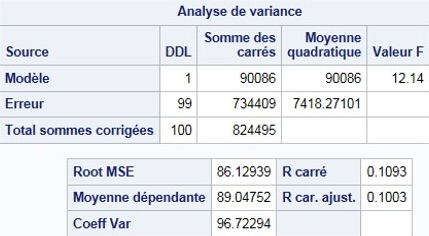
\includegraphics[scale=1.4]{Leinhardt_model1_SAA1.jpg}
\end{figure}\vspace{-0.5cm}
\begin{figure}[h!]
	\centering
	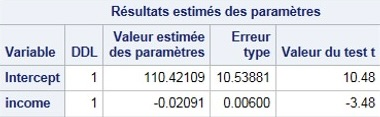
\includegraphics[scale=1.4]{Leinhardt_model1_SAS2.jpg}
\end{figure}

\newpage

On découvre ensuite que les postulats ne sont pas valides avec le modèle précédent. On transforme alors les variables pour ajuster le modèle suivant:
$$Y_i = \beta_0 + \beta_1 x_i + \varepsilon_i$$
avec $x_i $ le \underline{logarithme naturel} du revenu per capita en dollar américains du pays $i$ et $Y_i$ le \underline{logarithme naturel} du taux de mortalité infantile en décès par 1000 naissances du pays $i$. Voici des statistiques pour ce modèle, ainsi qu'une sortie R incomplète: 

\begin{verbatim}

Moyenne de la variable indépendante = 6.034396
Moyenne de la variable dépendante = 4.057454
S_xx = 179.7536


Coefficients:
               Estimate   Std. Error  t value   Pr(>|t|)    
(Intercept)       AAAA     0.31654     ????     <2e-16 
I(log(income)) -0.51179      BBBB     -9.992    <2e-16 
---
Residual standard error: 0.6867 on 99 degrees of freedom
Multiple R-squared:  0.5021,  Adjusted R-squared:  0.4971 


ANOVA

Response: I(log(infant))
               Df  Sum Sq  Mean Sq  F value    Pr(>F)    
I(log(income))  1  47.083   47.083   99.844   < 2.2e-16 
Residuals      99  46.685   0.472                      

\end{verbatim}

À l'aide de ces informations, répondez aux questions suivantes.

\vspace{0.1in}
	\part[3] En plus d'aider à améliorer la validité des postulats du modèle, donnez un signe que le deuxième modèle s'ajuste mieux aux données que le premier.
 \vspace{1.4 in}
 \part[2] Donnez la valeur de $S_{xy}$.
	\newpage
	\part[4] Calculez la valeur AAAA dans la sortie. 
	\vspace{1.9 in}
	\part[4] Calculez la valeur BBBB dans la sortie. 
	\vspace{1.9 in}
	\part[7] Soit un pays avec un revenu par capita de 1000 dollars américains. Donnez un intervalle à 99\% pour le taux de mortalité infantile dans ce pays.
	\vspace{1.5 in}
\end{parts}







\end{questions}




\end{document}




\vspace{0.3in}
\textbf{Question 4 (10 pts)} (Design d'expérience)\\

On s'intéresse à un médicament sensé réduire le nombre de crises chez les individus atteints d'epilepsie. Vous devez aider à planifier une expérience pour étudier l'effet de la dose du médicament sur le nombre de crises. Puisque vous vous intéressez à la relation entre deux variables quantitatives, vous planifiez analyser les données avec un modèle de régression linéaire simple. \\

Soit $x_1, \ldots, x_n$ les valeurs de la dose pour les 20 individus de votre étude.\\ Pour chacun, vous pouvez attribuer n'importe quelle dose entre 2 mg et 21 mg. \\

\begin{itemize}
%\item [(a)] Pour le modèle de régression linéaire simple $Y_i = \beta_0 + \beta_1 x_i + \varepsilon_i$, prouvez que la variance de $\beta_0$ est minimale si les $x_i$ sont tels que $\bar{x}$ = 0.
\item [(a)] (5 pts) Quelle est la meilleure fa\c{c}on de choisir les valeurs $x_1,\ldots,x_n$ pour minimiser la variance de votre estimateur $\hat{\beta_1}$? Justifiez votre réponse.
\vspace{0.1 in}
\item [(b)] (5 pts) Pourquoi ne serait-ce pas vraiment une bonne idée de choisir les valeurs de $x_i$ de cette façon, même si cela minimise la variance de votre estimateur?
\end{itemize}

\end{document} 